\documentclass[11pt, a4paper]{article}
\usepackage{amsfonts, amsmath, hanging, hyperref, natbib, parskip, times}
\usepackage[pdftex]{graphicx}
\hypersetup{
  colorlinks,
  linkcolor=blue,
  urlcolor=blue
}

\usepackage{wrapfig}

\let\section=\subsubsection
\newcommand{\pkg}[1]{{\normalfont\fontseries{b}\selectfont #1}} 
\let\proglang=\textit
\let\code=\texttt 
\renewcommand{\title}[1]{\begin{center}{\bf \LARGE #1}\end{center}}
\newcommand{\affiliations}{\footnotesize}
\newcommand{\keywords}{\paragraph{Keywords:}}

\setlength{\topmargin}{-15mm}
\setlength{\oddsidemargin}{-2mm}
\setlength{\textwidth}{165mm}
\setlength{\textheight}{250mm}

\begin{document}
\pagestyle{empty}

\title{\pkg{TriMatch}: An R Package for Propensity Score Matching of Non-Binary Treatments}

\begin{center}
  {\bf Jason M. Bryer$^{1,2,^\star}$}\\
  {\bf Kimberly K. Speerschneider$^{1,2}$}
\end{center}

\begin{affiliations}
1. University at Albany \\[-2pt]
2. Excelsior College \\[-2pt]
$^\star$Contact author: \href{mailto:jason@bryer.org}{jason@bryer.org}
\end{affiliations}

\keywords propensity score analysis, matching, non-binary treatments

\vskip 0.8cm

The use of propensity score methods \citep{RosenbaumRubin1983} have become popular for estimating causal inferences in observational studies in medical research \citep{Austin2008} and in the social sciences \citep{ThoemmesKim2011}. In most cases however, the use of propensity score methods have been confined to a single treatment. Several researchers have suggested using propensity score methods with multiple control groups, or to simply perform two separate analyses, one between treatment one and the control and another between treatment two and control. This talk introduces the \pkg{TriMatch} package for R that provides a method for determining matched triplets.  Examples from educational and medical contexts will be discussed.

\begin{wrapfigure}{r}{.4\textwidth}
    \vspace{0pt}
    \begin{center}
    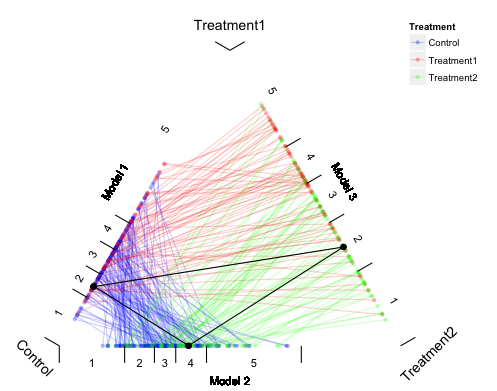
\includegraphics[width=.4\textwidth]{matches.png}
    \caption{Triangle Plot}
    \end{center}
    \label{trianglePlot}
    %\vspace{-50pt}
\end{wrapfigure}

Consider two treatments, $Tr_1$ and $Tr_2$, and a control, $C$. We estimate propensity scores with three separate logistic regression models where model one predicts $Tr_1$ with $C$, model two predicts $Tr_2$ with $C$, and model three predicts $Tr_1$ with $Tr_2$. The triangle plot in Figure 1 represents the fitted values (i.e. propensity scores) from the three models on each edge. Since each unit has a propensity score in two models, their scores are connected. The \pkg{TriMatch} algorithm will find matched triplets where the sum of the distances within each model is minimized. In Figure 1, the black lines illustrate one matched triplet.

%The first step in this approach for finding matched triplets involves estimating three propensity score models vis-\`{a}-vis logistic regression for each pair of groups (i.e. control-to-treatment one, control-to-treatment two, treatment one-to-treatment two). Starting with the larger of the two treatment groups, $Tr_1$, all elements from the smaller treatment, $Tr_2$, within a specified caliper (.25 of a standard deviation by default) are identified (using model 3 in Figure \ref{trianglePlot}). For each $Tr_2$ identified, control, $C$ elements from the within a specified caliper are identified (using model 2 in Figure \ref{trianglePlot}. Lastly, the distance between each $C$ unit and the originating $Tr_1$ unit is calculated (using model 1 in Figure 1). The total distance, the sum of distance between each pair, is calculated. The $m$ unique matches that minimize the total distance are returned.

Propensity score analysis of two groups typically use dependent sample \textit{t}-tests. The analogue for matched triplets include repeated measures ANOVA and the Freidman Rank Sum Test. The \pkg{TriMatch} package provides utility functions for conducting and visualizing these statistical tests. Moreover, a set of functions extending \pkg{PSAgraphics} \citep{HelmreichPruzek2008} for matched triplets to check covariate balance are provided.

%\begin{figure}[h!]
%\begin{center}
%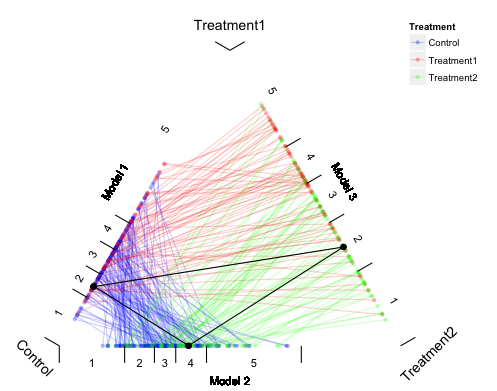
\includegraphics[height=2.75in]{matches.png}
%\caption{Triangle Plot Displaying with One Matched Triplet Overlayed}
%\label{fig:trimatch}
%\end{center}
%\end{figure}

%% references: 
%\nocite{ImaivanDyk2004,Zhaoetal2012}
\bibliographystyle{chicago}
\bibliography{TriMatch}

\end{document}
